\subsection{Circle Graphs}

\begin{definition}
\label{def:cgrid}
The $m \times n$ \term{comparability grid} is the graph
$\CGrid_{m\times n}=(V,E)$ with
\begin{align}
    V &= \{(i,j) \mid i \in [m],\ j \in [n]\}, \\
    E &= \bigl\{\{(i_1,j_1),(i_2,j_2)\} \mid
    (i_1,j_1)\neq (i_2,j_2),\
    (i_1-i_2)(j_1-j_2)\ge 0
    \bigr\}.
\end{align}
Equivalently, two distinct vertices are adjacent exactly when they are comparable
in the product order on $[m]\times[n]$. Denote this graph by $\CGrid_{m \times n}$. Let $\CGrid$ denote the family of all such graphs.
\end{definition}

\begin{example}
The figure below shows the $3 \times 3$ comparability grid:
\begin{figure}[H]
\centering
\begin{tikzpicture}[
  scale=1.7,
  every node/.style={circle, fill=black, inner sep=1.5pt},
  edge/.style={line width=0.5pt}
]
\node (v11) at (1,1) {};
\node (v12) at (1,2) {};
\node (v13) at (1,3) {};
\node (v21) at (2,1) {};
\node (v22) at (2,2) {};
\node (v23) at (2,3) {};
\node (v31) at (3,1) {};
\node (v32) at (3,2) {};
\node (v33) at (3,3) {};

\draw[edge] (v11) -- (v12);
\draw[edge] (v11) -- (v21);
\draw[edge] (v11) -- (v22);
\draw[edge] (v11) -- (v23);
\draw[edge] (v11) -- (v32);

\draw[edge] (v12) -- (v13);
\draw[edge] (v12) -- (v22);
\draw[edge] (v12) -- (v23);

\draw[edge] (v13) -- (v23);

\draw[edge] (v21) -- (v22);
\draw[edge] (v21) -- (v31);
\draw[edge] (v21) -- (v32);

\draw[edge] (v22) -- (v23);
\draw[edge] (v22) -- (v32);

\draw[edge] (v23) -- (v33);
\draw[edge] (v31) -- (v32);
\draw[edge] (v32) -- (v33);

\draw[edge] (v11) to[bend left=20] (v13);
\draw[edge] (v21) to[bend left=20] (v23);
\draw[edge] (v31) to[bend left=20] (v33);

\draw[edge] (v11) to[bend right=20] (v31);
\draw[edge] (v12) to[bend right=20] (v32);

\draw[edge] (v11) to[bend right=20] (v33);
\draw[edge] (v12) to[bend right=20] (v33);
\draw[edge] (v13) to[bend right=20] (v33);

\draw[edge] (v21) to[bend right=20] (v33);
\draw[edge] (v22) to[bend right=20] (v33);

\node[draw=none, fill=none, inner sep=0pt, anchor=east] at ($(v13)+(-0.15,0)$) {$ (1,3)$};
\node[draw=none, fill=none, inner sep=0pt, anchor=west] at ($(v33)+(0.15,0)$) {$ (3,3)$};
\node[draw=none, fill=none, inner sep=0pt, anchor=east] at ($(v11)+(-0.15,0)$) {$ (1,1)$};
\node[draw=none, fill=none, inner sep=0pt, anchor=west] at ($(v31)+(0.15,0)$) {$ (3,1)$};
\end{tikzpicture}
\label{fig:comp-grid-example}
\caption{$\CGrid_{3 \times 3}$.}
\end{figure}

\end{example}

Comparability grids are also circle graphs.

\begin{definition}
\label{def:circle-graph}
A \term{circle graph} is an intersection graph of chords of a circle. Equivalently, a graph $G = (V,E)$ is a circle graph if we can assign each $v \in V$ a chord $c_v$ in a circle such that 
\begin{align}
    uv \in E \iff c_u \text{ and } c_v \text{ intersect}.
\end{align}
Denote the family of all circle graphs as $\CGraph$.
\end{definition}

To see that comparability graphs are circle graphs, we introduce another kind of circle graph: permutation graphs.

\begin{definition}
\label{def:permutation-graph}
A \term{permutation graph} is a graph that records which pairs of objects are in opposite order in two different lists. More precisely, let $V$ be a finite set of labels, and choose two total orders $<_1$ and $<_2$ on $V$. The permutation graph $G = (V,E)$ associated with these two orders has $V$ as its vertices, and edges
\begin{align}
    uv \in E \iff (u <_1 v \land v <_2 u) \lor (v <_1 u \land u <_2 v).
\end{align}
To draw a permutation graph, place the vertices in $<_1$ order on one horizontal line, and place the vertices in $<_2$ order on a second horizontal line below it. Connect matching labels with a line segment. Then two vertices are adjacent exactly when their line segments cross. Denote the family of all permutation graphs as $\PGraph$.
\end{definition}

\begin{figure}[H]
\centering

\begin{minipage}{0.48\textwidth}
\centering
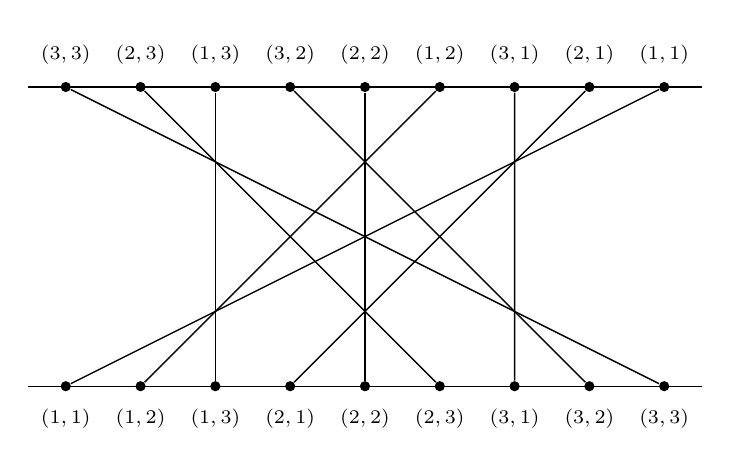
\begin{tikzpicture}[
    scale=0.95,
    every node/.style={circle, fill=black, inner sep=1.3pt},
    edge/.style={line width=0.5pt},
    lab/.style={draw=none, fill=none, inner sep=0pt, font=\scriptsize}
]
\draw[line width=0.5pt] (0.5,0) -- (9.5,0);
\draw[line width=0.5pt] (0.5,4) -- (9.5,4);

\node (b11) at (1,0) {};
\node (b12) at (2,0) {};
\node (b13) at (3,0) {};
\node (b21) at (4,0) {};
\node (b22) at (5,0) {};
\node (b23) at (6,0) {};
\node (b31) at (7,0) {};
\node (b32) at (8,0) {};
\node (b33) at (9,0) {};

\node (t33) at (1,4) {};
\node (t23) at (2,4) {};
\node (t13) at (3,4) {};
\node (t32) at (4,4) {};
\node (t22) at (5,4) {};
\node (t12) at (6,4) {};
\node (t31) at (7,4) {};
\node (t21) at (8,4) {};
\node (t11) at (9,4) {};

\draw[edge] (b11) -- (t11);
\draw[edge] (b12) -- (t12);
\draw[edge] (b13) -- (t13);
\draw[edge] (b21) -- (t21);
\draw[edge] (b22) -- (t22);
\draw[edge] (b23) -- (t23);
\draw[edge] (b31) -- (t31);
\draw[edge] (b32) -- (t32);
\draw[edge] (b33) -- (t33);

\node[lab, below=2pt] at (b11) {$(1,1)$};
\node[lab, below=2pt] at (b12) {$(1,2)$};
\node[lab, below=2pt] at (b13) {$(1,3)$};
\node[lab, below=2pt] at (b21) {$(2,1)$};
\node[lab, below=2pt] at (b22) {$(2,2)$};
\node[lab, below=2pt] at (b23) {$(2,3)$};
\node[lab, below=2pt] at (b31) {$(3,1)$};
\node[lab, below=2pt] at (b32) {$(3,2)$};
\node[lab, below=2pt] at (b33) {$(3,3)$};

\node[lab, above=2pt] at (t33) {$(3,3)$};
\node[lab, above=2pt] at (t23) {$(2,3)$};
\node[lab, above=2pt] at (t13) {$(1,3)$};
\node[lab, above=2pt] at (t32) {$(3,2)$};
\node[lab, above=2pt] at (t22) {$(2,2)$};
\node[lab, above=2pt] at (t12) {$(1,2)$};
\node[lab, above=2pt] at (t31) {$(3,1)$};
\node[lab, above=2pt] at (t21) {$(2,1)$};
\node[lab, above=2pt] at (t11) {$(1,1)$};

% \node[lab] at (5,-0.8) {bottom order: $(1,1),(1,2),(1,3),(2,1),(2,2),(2,3),(3,1),(3,2),(3,3)$};
% \node[lab] at (5,4.8) {top order: $(3,3),(2,3),(1,3),(3,2),(2,2),(1,2),(3,1),(2,1),(1,1)$};
\end{tikzpicture}
\end{minipage}
\hfill
\begin{minipage}{0.48\textwidth}
\centering
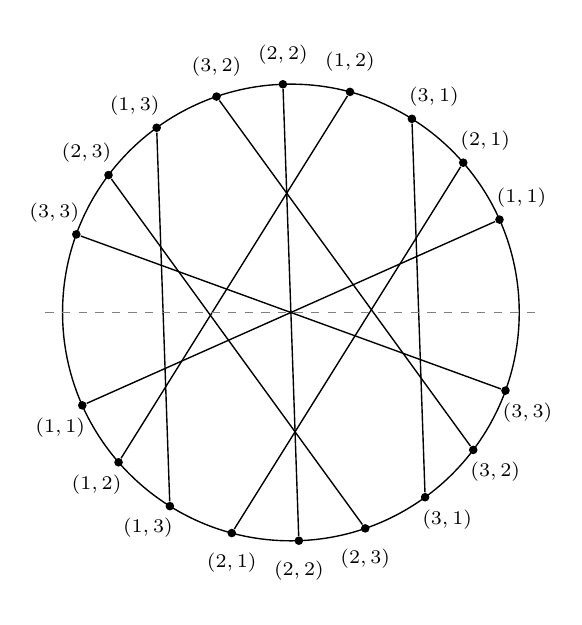
\begin{tikzpicture}[
    scale=1.45,
    every node/.style={circle, fill=black, inner sep=1.1pt},
    edge/.style={line width=0.5pt},
    lab/.style={draw=none, fill=none, inner sep=0pt, font=\scriptsize}
]
\draw[line width=0.5pt] (0,0) circle (2);

\node (u1) at (160:2) {};
\node (u2) at (143:2) {};
\node (u3) at (126:2) {};
\node (u4) at (109:2) {};
\node (u5) at (92:2)  {};
\node (u6) at (75:2)  {};
\node (u7) at (58:2)  {};
\node (u8) at (41:2)  {};
\node (u9) at (24:2)  {};

\node (d1) at (204:2) {};
\node (d2) at (221:2) {};
\node (d3) at (238:2) {};
\node (d4) at (255:2) {};
\node (d5) at (272:2) {};
\node (d6) at (289:2) {};
\node (d7) at (306:2) {};
\node (d8) at (323:2) {};
\node (d9) at (340:2) {};

\draw[edge] (u9) -- (d1);
\draw[edge] (u6) -- (d2);
\draw[edge] (u3) -- (d3);
\draw[edge] (u8) -- (d4);
\draw[edge] (u5) -- (d5);
\draw[edge] (u2) -- (d6);
\draw[edge] (u7) -- (d7);
\draw[edge] (u4) -- (d8);
\draw[edge] (u1) -- (d9);

\node[lab, above left=1pt]  at (u1) {$(3,3)$};
\node[lab, above left=1pt]  at (u2) {$(2,3)$};
\node[lab, above left=1pt]  at (u3) {$(1,3)$};
\node[lab, above=1pt]       at (u4) {$(3,2)$};
\node[lab, above=1pt]       at (u5) {$(2,2)$};
\node[lab, above=1pt]       at (u6) {$(1,2)$};
\node[lab, above right=1pt] at (u7) {$(3,1)$};
\node[lab, above right=1pt] at (u8) {$(2,1)$};
\node[lab, above right=1pt] at (u9) {$(1,1)$};

\node[lab, below left=1pt]  at (d1) {$(1,1)$};
\node[lab, below left=1pt]  at (d2) {$(1,2)$};
\node[lab, below left=1pt]  at (d3) {$(1,3)$};
\node[lab, below=1pt]       at (d4) {$(2,1)$};
\node[lab, below=1pt]       at (d5) {$(2,2)$};
\node[lab, below=1pt]       at (d6) {$(2,3)$};
\node[lab, below right=1pt] at (d7) {$(3,1)$};
\node[lab, below right=1pt] at (d8) {$(3,2)$};
\node[lab, below right=1pt] at (d9) {$(3,3)$};

\draw[dashed, gray] (-2.15,0) -- (2.15,0);

\end{tikzpicture}
\end{minipage}
\caption{A permutation graph representation of $\CGrid_{3\times 3}$ and the equivalent circle graph representation.}
\label{fig:perm-to-circle-cgrid}
\end{figure}

\begin{theorem}
\label{thm:cgrid-is-perm-is-circle}
A comparability grid is a permutation graph, and hence a circle graph.
\end{theorem}

\begin{proof}
Fix a $G = \CGrid_{m \times n}$. Apply the perturbation from \ref{fact:tuple-construction}. This perturbation makes all first coordinates distinct and all second coordinates distinct. Now, define two orders on $V(G)$:
\begin{align}
    (i,j) <_1 (i',j') &\iff i < i' \lor (i = i' \land j < j') \\
    (i,j) <_2 (i',j') &\iff j > j' \lor (j = j' \land i > i')
\end{align}
These are lexicographic orders and thus total orders. Now, draw a permutation diagram with vertices on the top line in order $<_2$ and $<_1$ on the bottom line. Connect equal labels with a line segment. Since the second order is reversed, the two segments cross exactly when the first and second coordinate differences have the same sign. Hence $G$ is a permutation graph.

Finally, we show that any permutation graph is a circle graph. Place the two parallel lines of a permutation graph inside a circle and identify their endpoints along the boundary, such that each line segment becomes a chord of a circle. This preserves crossings. Therefore every permutation graph is a circle graph.
\end{proof}

\begin{theorem}
\label{thm:circle-graph-lu-equals-lc}
This is Theorem 1 of \cite{circle-graphs}. For circle graph states, $\LU = \LC$. Furthermore, the only graphs $\LU$-equivalent to circle graph states are circle graphs themselves. Since local complementation of graph states is implemented by local Clifford
operations, and local Clifford operations are local unitaries, this implies that $\CGraph$ is closed under local complementation.
\end{theorem}

\begin{definition}
\label{def:vertex-minor}
A graph $H$ is a \term{vertex-minor} of a graph $G$ if there is a sequence of vertex deletions and local complementations from $G$ to $H$.
\end{definition}

\begin{proof}
By Theorem \ref{thm:circle-graph-lu-equals-lc}, circle graphs are closed under
local complementation. They are also closed under vertex deletion, since deleting
a vertex from the intersection graph corresponds to deleting the corresponding
chord from the chord diagram.
\end{proof}

\begin{proof}
This follows from Theorem \ref{thm:circle-graph-lu-equals-lc}.
\end{proof}

\begin{theorem}
\label{thm:cgraph-vertex-minor-bipartite-cgraph}
This follows from Corollary 53 of \cite{brijder2016isotropicmatroidsiicircle}, together with the strengthening in \cite{circle-graphs}. Every circle graph is a vertex-minor of some bipartite circle graph that is at most quadratically larger in the number of vertices.
\end{theorem}

\begin{theorem}
\label{thm:cgraph-vertex-minor-cgrid}
This is Lemma 3.1, 3.2, and 3.3 of \cite{grid-theorem}. Every circle graph on $n$ vertices is isomorphic to a vertex-minor of the $3n \times 3n$ comparability grid. More specifically, every $n$-vertex permutation graph is isomorphic to an induced subgraph of the $n \times n$ comparability grid, and every circle graph on $n$ vertices is a vertex-minor of a permutation graph on $3n$ vertices.
\end{theorem}

\begin{theorem}
\label{thm:cgrid-efficiently-simulable}
This follows from Corollaries 3 and 4 of \cite{circle-graphs}. MBQC on circle graph states is efficiently classically simulable. Furthermore, assuming $\BPP \neq \BQP$\footnote{\term{$\BPP$} is the classical complexity class for bounded polynomial-time, defined in \cite{bpp-def}. \term{$\BQP$} is the quantum complexity class for bounded-error quantum polynomial-time, defined in \cite{bqp-def}}, polynomial rank-width is not a sufficient condition for efficient universality of a graph state resources for MBQC.
\end{theorem}

The previous theorem begins to highlight connections between rank-width and circle graphs. Restricting our attention to comparability grids, we observe even more connections.

\begin{theorem}
\label{thm:cgrid-unbounded-rank-width}
The rank-width of the $n \times n$ comparability grid is at least $n/4$. Thus, $\CGrid$ has unbounded rank-width, and so do $\PGraph$ and $\CGraph$.
\end{theorem}

\begin{proof}
The first claim is Lemma 4 of \cite{circle-graphs}. The second follows by Theorem \ref{thm:cgrid-is-perm-is-circle}.
\end{proof}

\begin{theorem}
\label{thm:rank-width-vertex-minor-cgrid}
This is Theorem 1.1 and 1.3 of \cite{GEELEN202393}. There is a function $f: \N \to \N$ such that for every positive integer $n$, every graph of rank-width at least $f(n)$ has a vertex-minor isomorphic to the $n \times n$ comparability grid. On the other hand, there is a function $g: \N \to \N$ such that for every circle graph $H$, every graph with no vertex-minor isomorphic to $H$ has rank-width at most $g(|V(H)|)$.
\end{theorem}

We conclude this section by contrasting the above results for circle graphs and comparability grids with a result for grid graphs.

\begin{theorem}
\label{thm:every-graph-vertex-minor-of-grid}
This is Theorem 12 and 19 of \cite{campbell2024treewidthhadwigernumberinduced}. Every planar graph is a vertex-minor of some regular grid. Furthermore, every graph is a vertex-minor of some planar graph. Thus every graph is a vertex-minor of some regular grid.
\end{theorem}

This is in sharp contrast with the following result.

\begin{theorem}
\label{thm:forbidden-minor-of-cgraph}
This is the main result of \cite{BOUCHET1994107}. A graph $G$ is a circle graph if and only if no graph locally equivalent to $G$
has an induced subgraph isomorphic to one of the graphs below. These are known as the \term{forbidden vertex-minors} of circle graphs (and consequently, by Theorem \ref{thm:cgraph-vertex-minor-cgrid}, of comparability grids).
\begin{figure}[H]
    \centering
    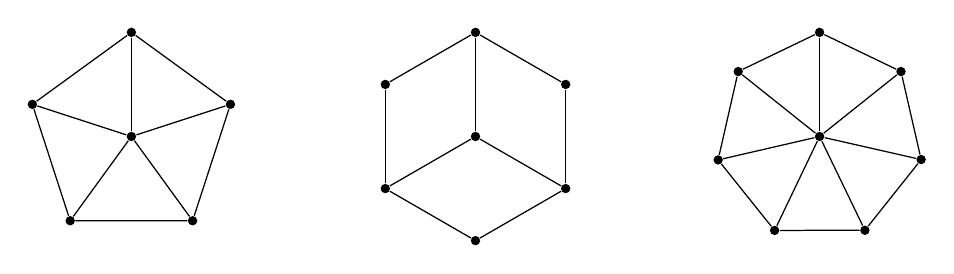
\begin{tikzpicture}[
        scale=1.15,
        vertex/.style={circle, fill=black, inner sep=1.2pt},
        edge/.style={line width=0.45pt}
    ]
    
    % Left graph
    \begin{scope}[xshift=0cm]
        \foreach \i/\ang in {1/90,2/18,3/-54,4/-126,5/162}
            \node[vertex] (a\i) at (\ang:1.15) {};
        \node[vertex] (ac) at (0,0) {};
    
        \foreach \i/\j in {1/2,2/3,3/4,4/5,5/1}
            \draw[edge] (a\i) -- (a\j);
        \foreach \i in {1,2,3,4,5}
            \draw[edge] (ac) -- (a\i);
    \end{scope}
    
    % Middle graph
    \begin{scope}[xshift=3.8cm]
        \foreach \i/\ang in {1/90,2/30,3/-30,4/-90,5/-150,6/150}
            \node[vertex] (b\i) at (\ang:1.15) {};
        \node[vertex] (bc) at (0,0) {};
    
        \foreach \i/\j in {1/2,2/3,3/4,4/5,5/6,6/1}
            \draw[edge] (b\i) -- (b\j);
        \foreach \i in {1,3,5}
            \draw[edge] (bc) -- (b\i);
    \end{scope}
    
    % Right graph
    \begin{scope}[xshift=7.6cm]
        \foreach \i/\ang in {1/90,2/38.6,3/-12.8,4/-64.2,5/-115.6,6/-167,7/141.4}
            \node[vertex] (c\i) at (\ang:1.15) {};
        \node[vertex] (cc) at (0,0) {};
    
        \foreach \i/\j in {1/2,2/3,3/4,4/5,5/6,6/7,7/1}
            \draw[edge] (c\i) -- (c\j);
        \foreach \i in {1,2,3,4,5,6,7}
            \draw[edge] (cc) -- (c\i);
    \end{scope}
    
    \end{tikzpicture}
    \caption{Forbidden vertex minors of circle grpahs.}
    \end{figure}
\end{theorem}